%!TEX root = ../main.tex

\section{Backgrounds (2 pages)}
\label{sec:bd2jpsiks:backgrounds}

Although \BdToJPsiKS is an experimentally very clean decay channel care has to
be taken to properly identify, suppress or even reject backgrounds. While the
two muons can be identified quite effectively the pions of the \KS decay might
actually be kaons or protons, which have been mis-identified. This would lead
to background contributions from \BdToJPsiKst and \LbToJPsiL. To analyse the
$\proton \to \pion$ mis-ID the proton mass hypothesis is assigned to one of
the pions and the invariant mass of the proton-pion pair $m_{\proton\pion}$ is
recalculated. An excess of candidates at the \Lz mass $M_{\Lz} =
\SI{1115.683}{\MeVcc}$~\cite{PDG2014} can be seen, which is reduced by applying
a tighter requirement on the difference of the proton-pion log-likelihood for
candidates close to $M_{\Lz}$. With \LbToJPsiL signal MC it is checked that
after reconstruction, stripping and all offline selection requirements,
including the veto described above, the expected yield is a sub-percent
effect. For $\kaon \to \pion$ mis-ID the broad width of the \Kstarz does not
allow an analogous approach. But studies on \BdToJPsiKst MC show that the
expected contribution is even lower than for \LbToJPsiL. The main reason is
the short lifetime of the \Kstarz, which is exploited by the lifetime
significance cut on the \KS. So, it can basically be assumed that besides the
signal candidates almost only combinatorial background is present in the data
sample. Nevertheless, it has to be studied whether the background shows any
tagging-dependent asymmetry, which would dilute the measured \CP asymmetry.

By performing a fit to the invariant mass distribution the \sPlot technique
provides a possibility to study the tagging-dependent distributions of the
combinatorial background. First of all, the time-integrated asymmetry
\begin{align}
  \mathcal{A}_\text{bkg}^{\text{int}} = \frac{\param{N}{\Bzb}{bkg} - \param{N}{\Bz}{bkg}}{\param{N}{\Bzb}{bkg} + \param{N}{\Bz}{bkg}}
\end{align}
is calculated for both track type categories and separately for the OS tagging
combination and the SS\pion tagging algorithm. Out of the four values listed
in \cref{tab:bkgtimeintegratedasymm} only the one for the downstream OS tagged
sample, which has the highest statistics, stands out as it disfavours \CP
symmetry at more than \num{3} standard deviations.
%
\begin{table}[!htb]
\centering
\caption{Time-integrated asymmetry of sweighted background distributions for
downstream and long track OS and SS\pion tagged events.}
\label{tab:bkgtimeintegratedasymm}
\begin{tabular}{lr@{$\,\pm\,$}l}
	\toprule
category    & \multicolumn{2}{c}{$\mathcal{A}_\text{bkg}^{\text{int}}$}\\
\midrule
DD OS       & $0.017$     & $0.005$ \\
DD SS\pion  & $-0.016$    & $0.011$ \\
LL OS       & $-0.005$    & $0.012$ \\
LL SS\pion  & $0.044$     & $0.034$ \\
\bottomrule
\end{tabular}
\end{table}
%
But even time-integrated asymmetries compatible with zero do not exclude
time-dependent asymmetries. The latter are investigated by dividing the data
sample in ten bins of the decay time. The bin size is chosen to increase
exponentially. In \cref{fig:background_asymmetry_sweighted} again the four
categories of before are plotted.
%
\begin{figure}[!htb]
\centering
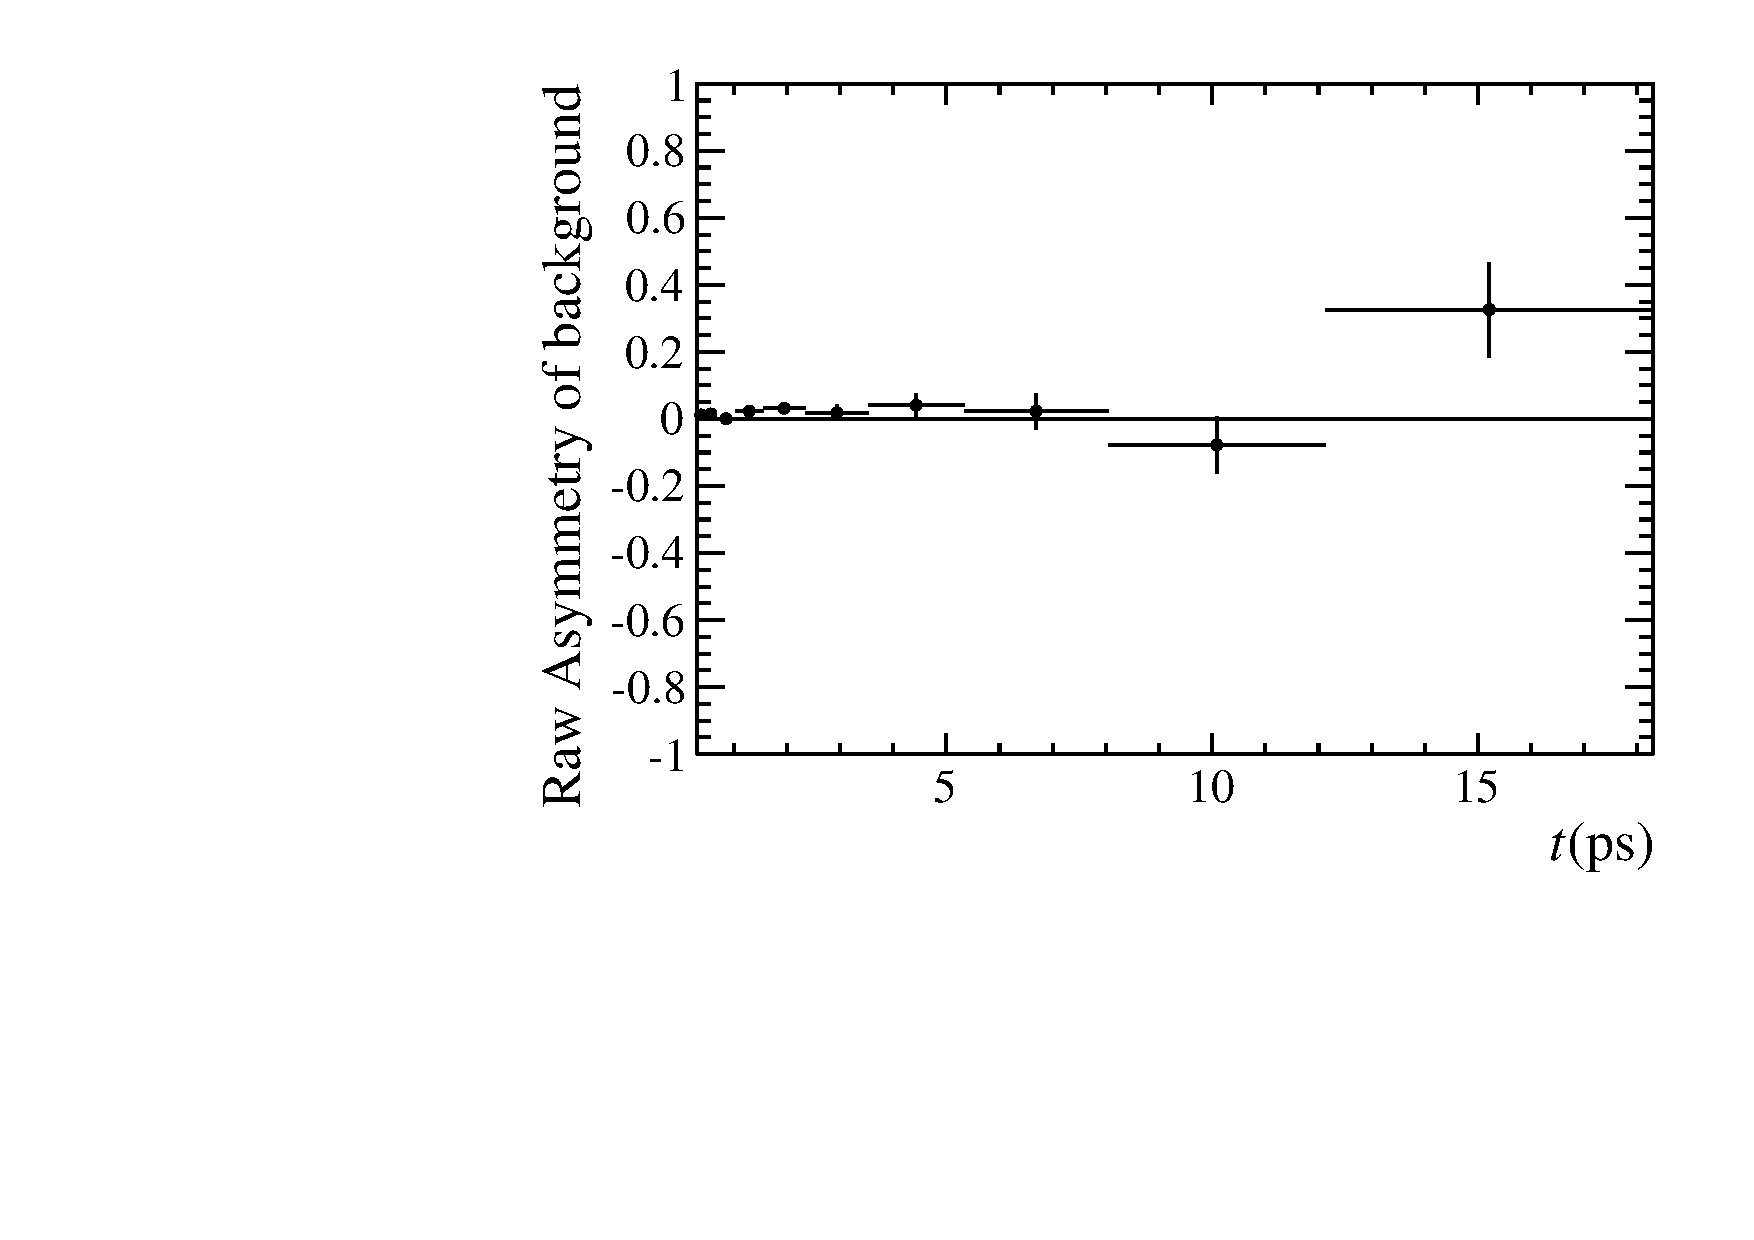
\includegraphics[width=0.49\textwidth]{06-Bd2JpsiKS/figs/BackgroundAsymmetryByHand_DD_OS_data.pdf}
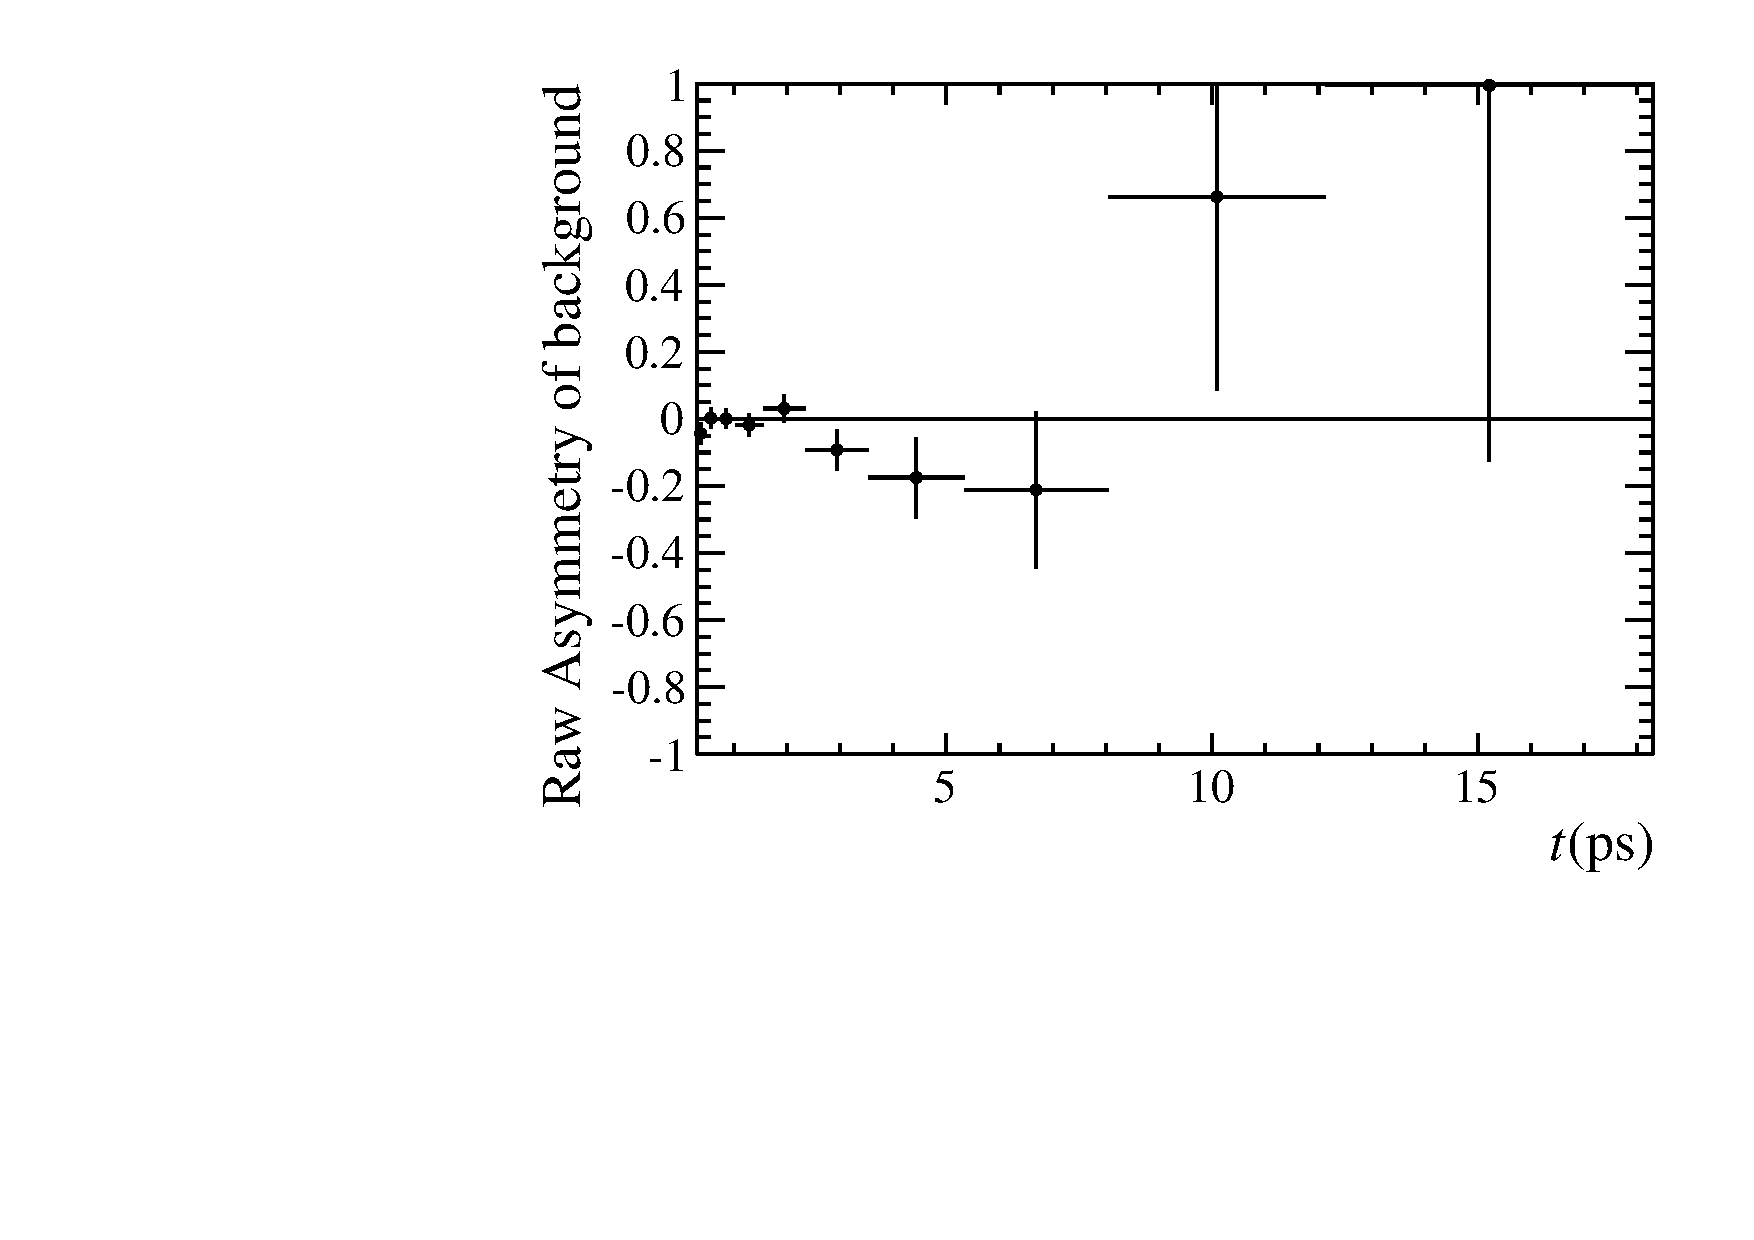
\includegraphics[width=0.49\textwidth]{06-Bd2JpsiKS/figs/BackgroundAsymmetryByHand_DD_SSPion_data.pdf}\\
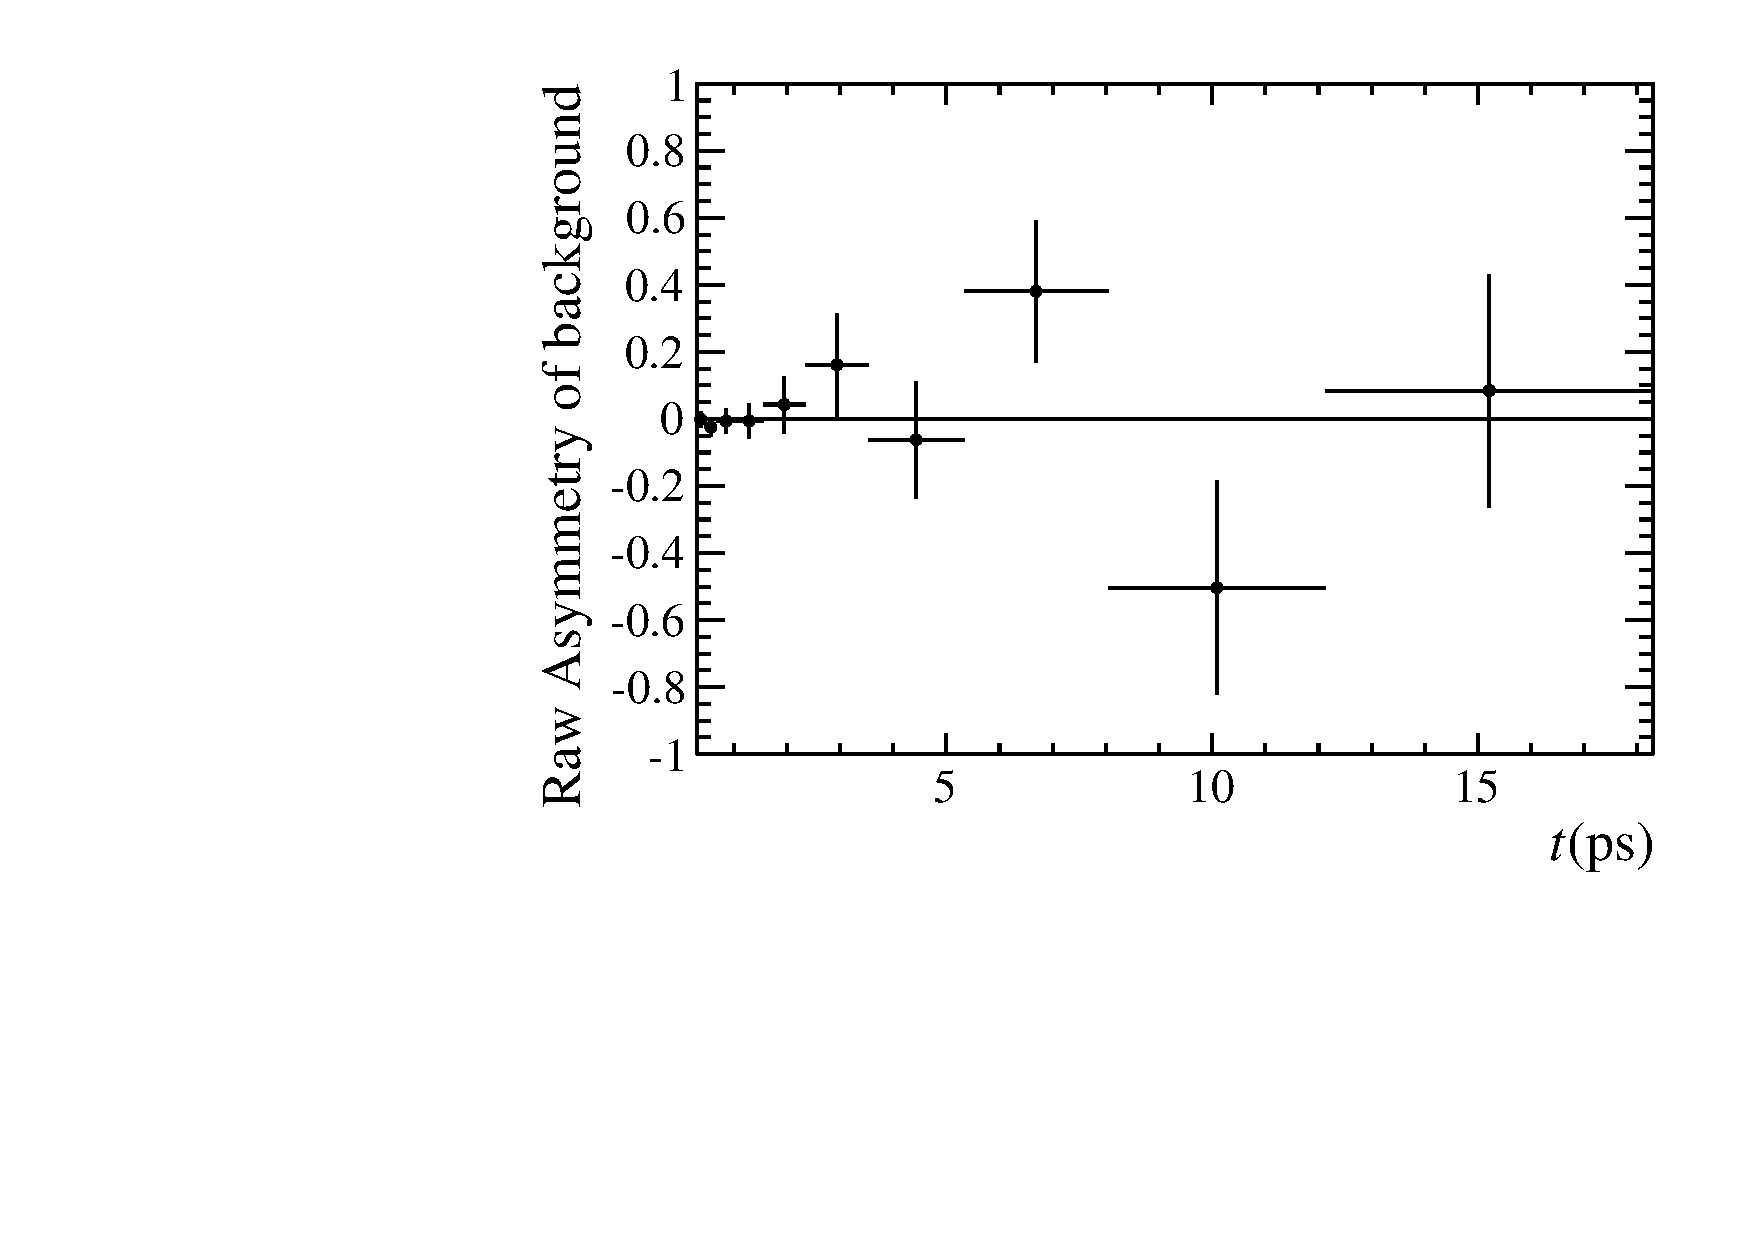
\includegraphics[width=0.49\textwidth]{06-Bd2JpsiKS/figs/BackgroundAsymmetryByHand_LL_OS_data.pdf}
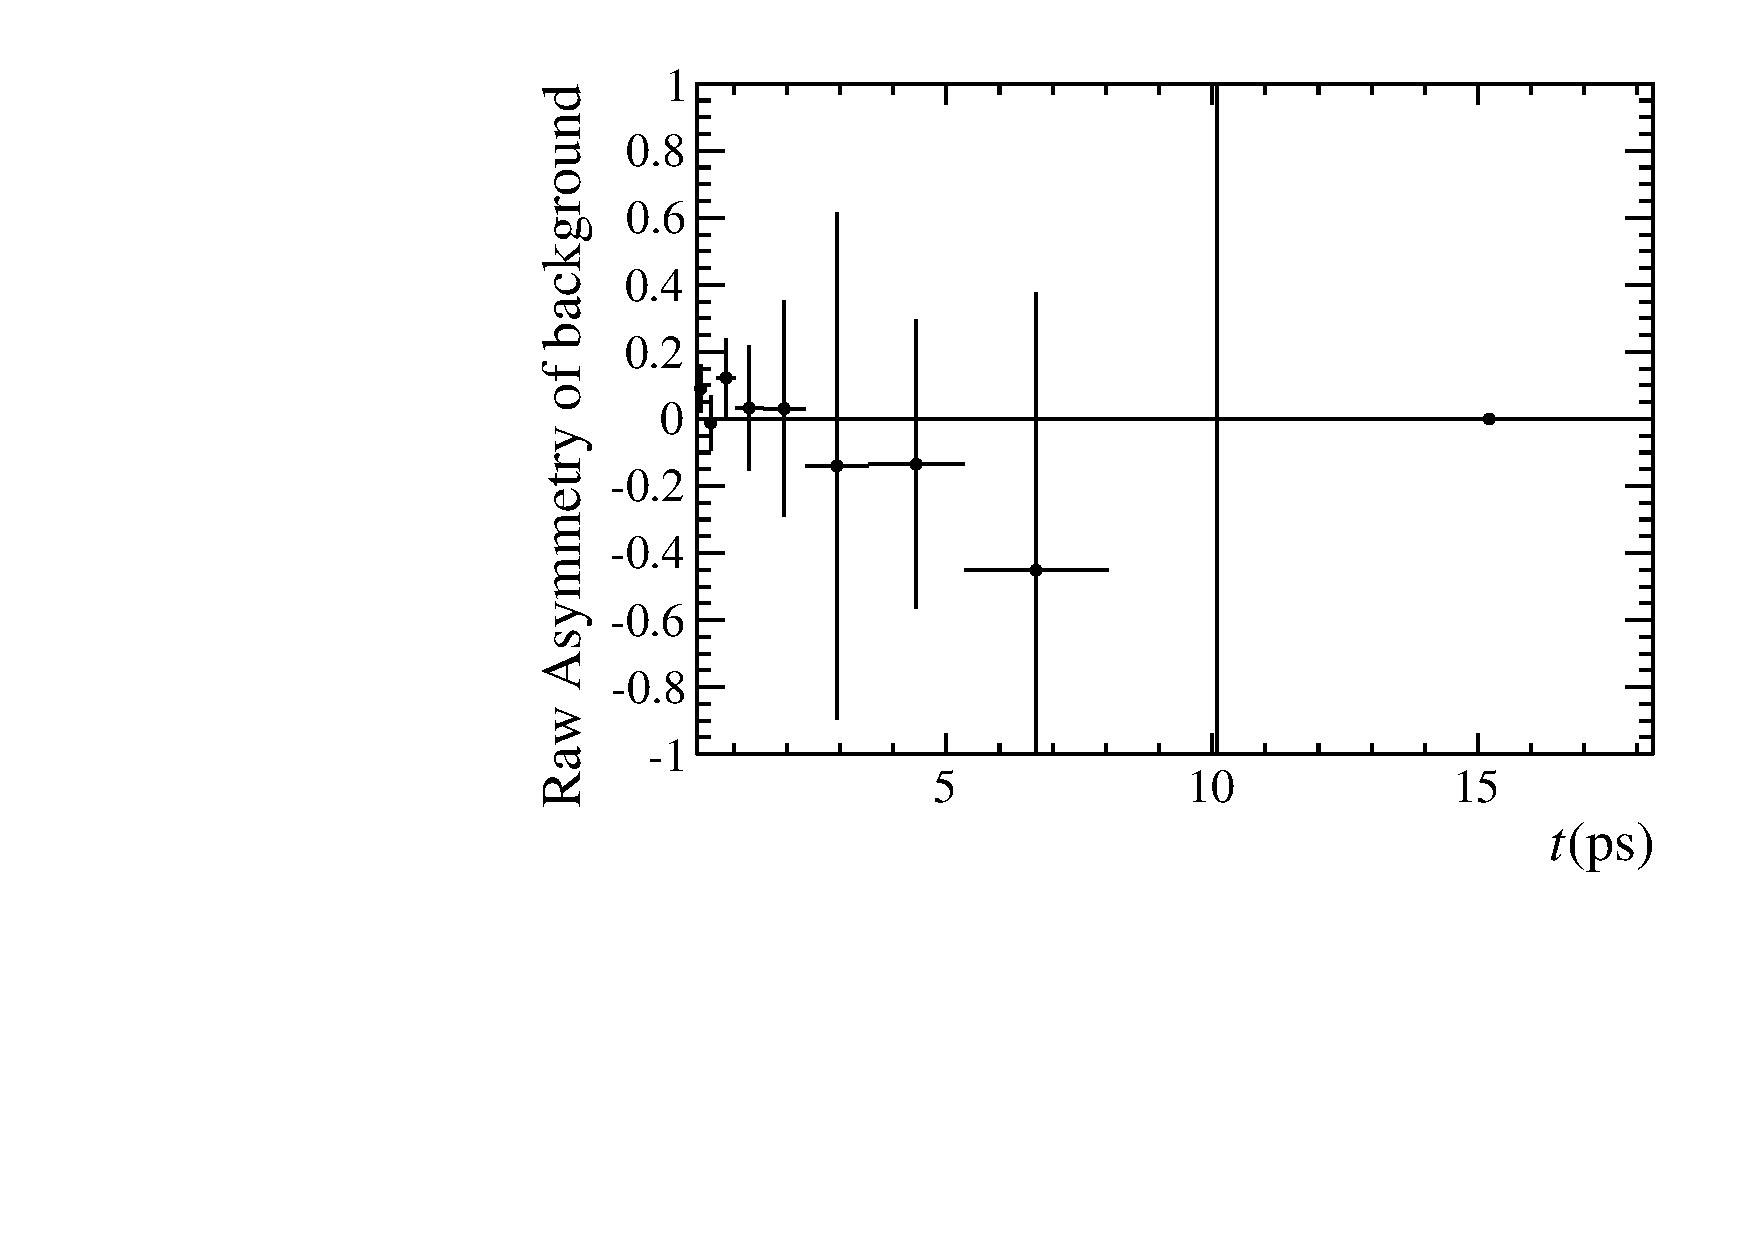
\includegraphics[width=0.49\textwidth]{06-Bd2JpsiKS/figs/BackgroundAsymmetryByHand_LL_SSPion_data.pdf}
\caption{Raw background asymmetry in sweighted data with logarithmic binning.
DD on top, LL on bottom plots. OS tagged candidates on the left, SS\pion tagged
candidates on the right side.}
\label{fig:background_asymmetry_sweighted}
\end{figure}
%
It's difficult to judge by eye if there is a significant oscillation. So,
\chisq-tests against the null-hypothesis, \ie a flat line at zero, are
performed and the corresponding $p$-values are calculated. The results are
\num{0.100} for DD OS, \num{0.437} for DD SS, \num{0.617} for DD SS, and
\num{0.969} for LL OS. None of the $p$-values is very low so the deviations
from zero can be explained with statistical fluctuations. The same procedure
(mass fit \to sWeights \to histograms of $\mathcal{A}_{\text{bkg}}$) is
performed with cocktail MC consisting of signal MC and background Toy MC.
Here, no asymmetry is generated for the background and the resulting
$p$-values are very similar to the ones for the nominal data sample. Finally,
an unbinned likelihood fit is performed to the sweighted background decay time
distribution using two/three exponentials with different pseudo-lifetimes and
allowing for tagging-dependent asymmetries in the PDF. All asymmetry
parameters are compatible with zero at a significance of two standard
deviations.